\chapter{Model Description}
\label{ch:chapter4}
As mentioned in Chapter 1, I am using a model of the \Gls{msbr}
\cite{robertson_conceptual_1971} to verify my \OpenMC implementation in
\SaltProc.

I picked the \Gls{msbr} because\ldots 

\section{Description of MSBR}
\label{sec:msbr_spec}

The \Gls{msbr} design is the result of a design study of a single-fluid
\Gls{msr} following the success of the \Gls{msre}
\cite{haubenreich_experience_1970}\cite{rosenthal_molten-salt_1970}.
I will only describe the following reactor systems that are relevant to
my validation study\footnote{A complete description of the entire \Gls{msbr}
system can be found in \cite{robertson_conceptual_1971}}: the fuel salt, the
reactor core, and the salt reprocessing system.

\begin{figure}[htpb]
    \centering
    \subfloat[][]{
        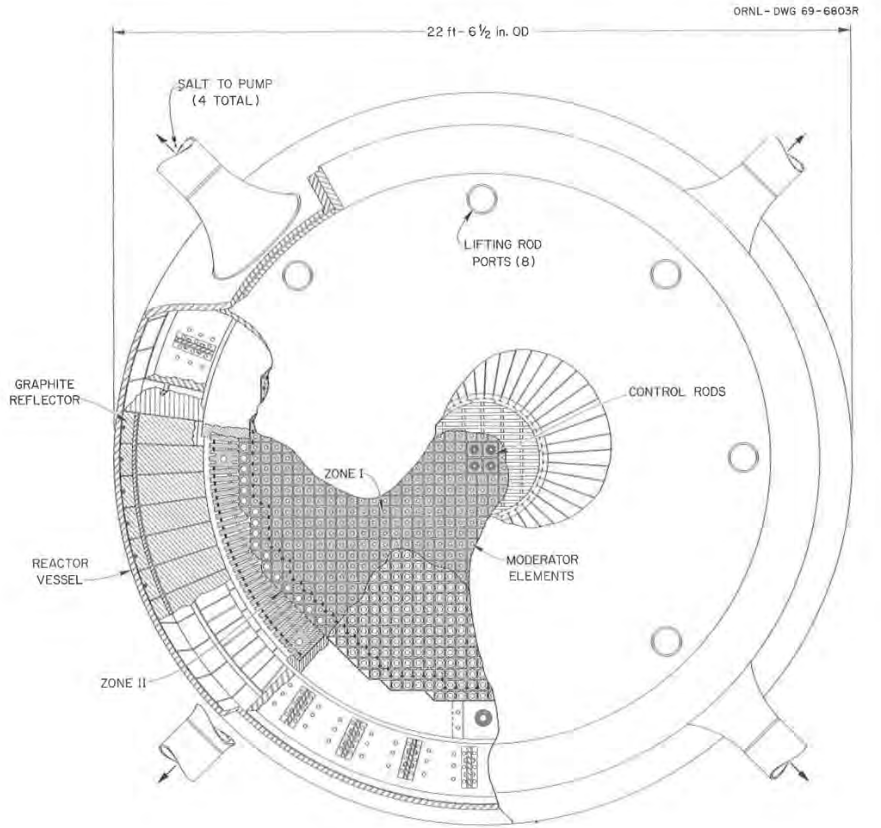
\includegraphics[width=0.5\linewidth]{figs/ch4/msbr_full_xy_ref.png}
        \label{fig:msbr_ref_xy}
    }
    \subfloat[][]{
        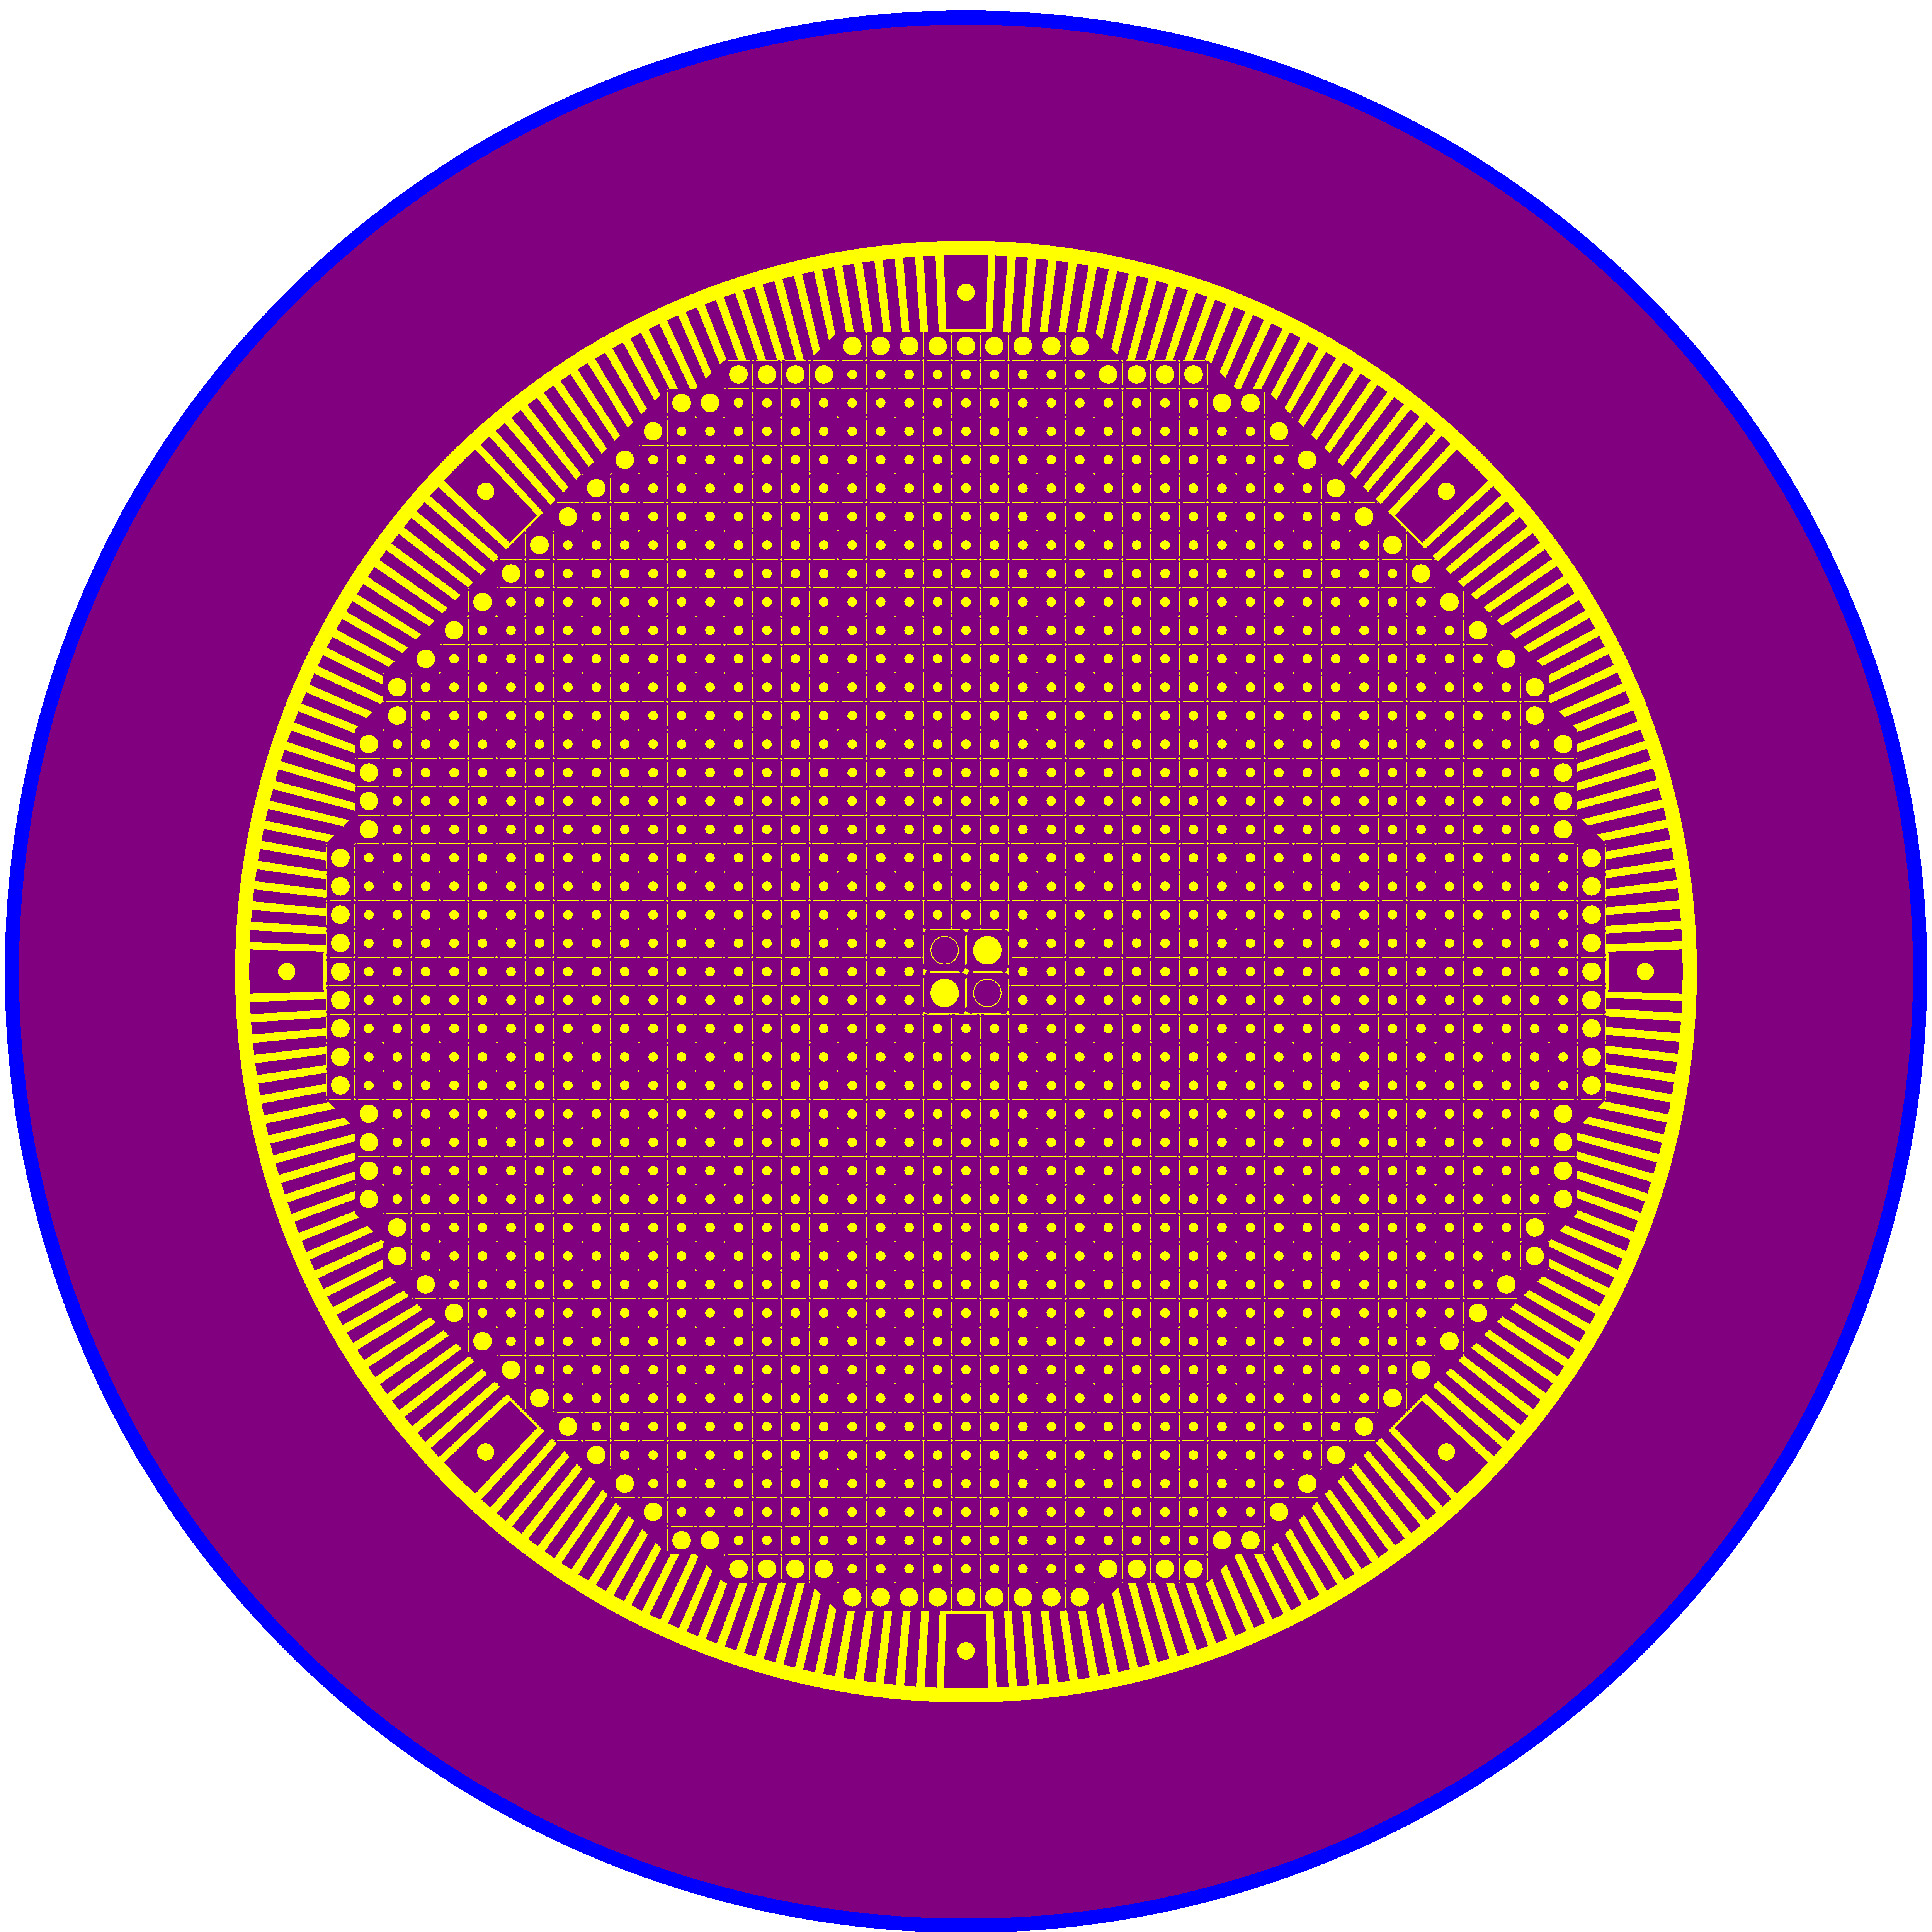
\includegraphics[width=0.5\linewidth]{figs/ch4/msbr_full_xy_openmc.png}
        \label{fig:msbr_model_xy}
    }
    \\
    \subfloat[][]{
        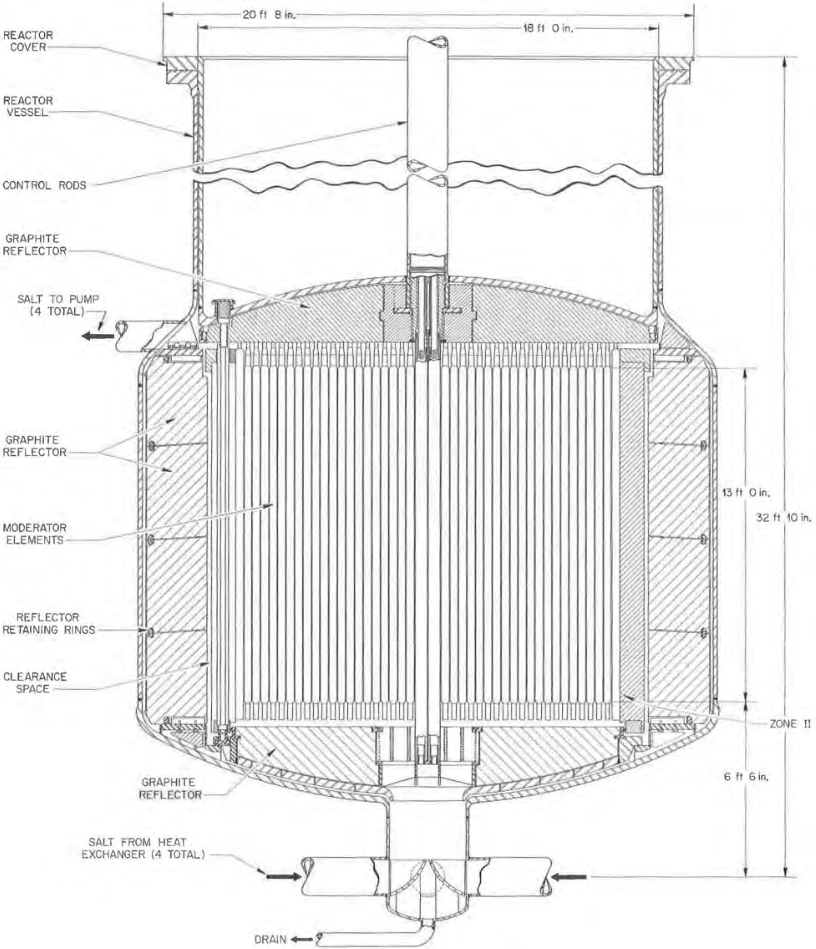
\includegraphics[width=0.5\linewidth]{figs/ch4/msbr_full_xz_ref.png}
        \label{fig:msbr_ref_xz}
    }
    \subfloat[][]{
        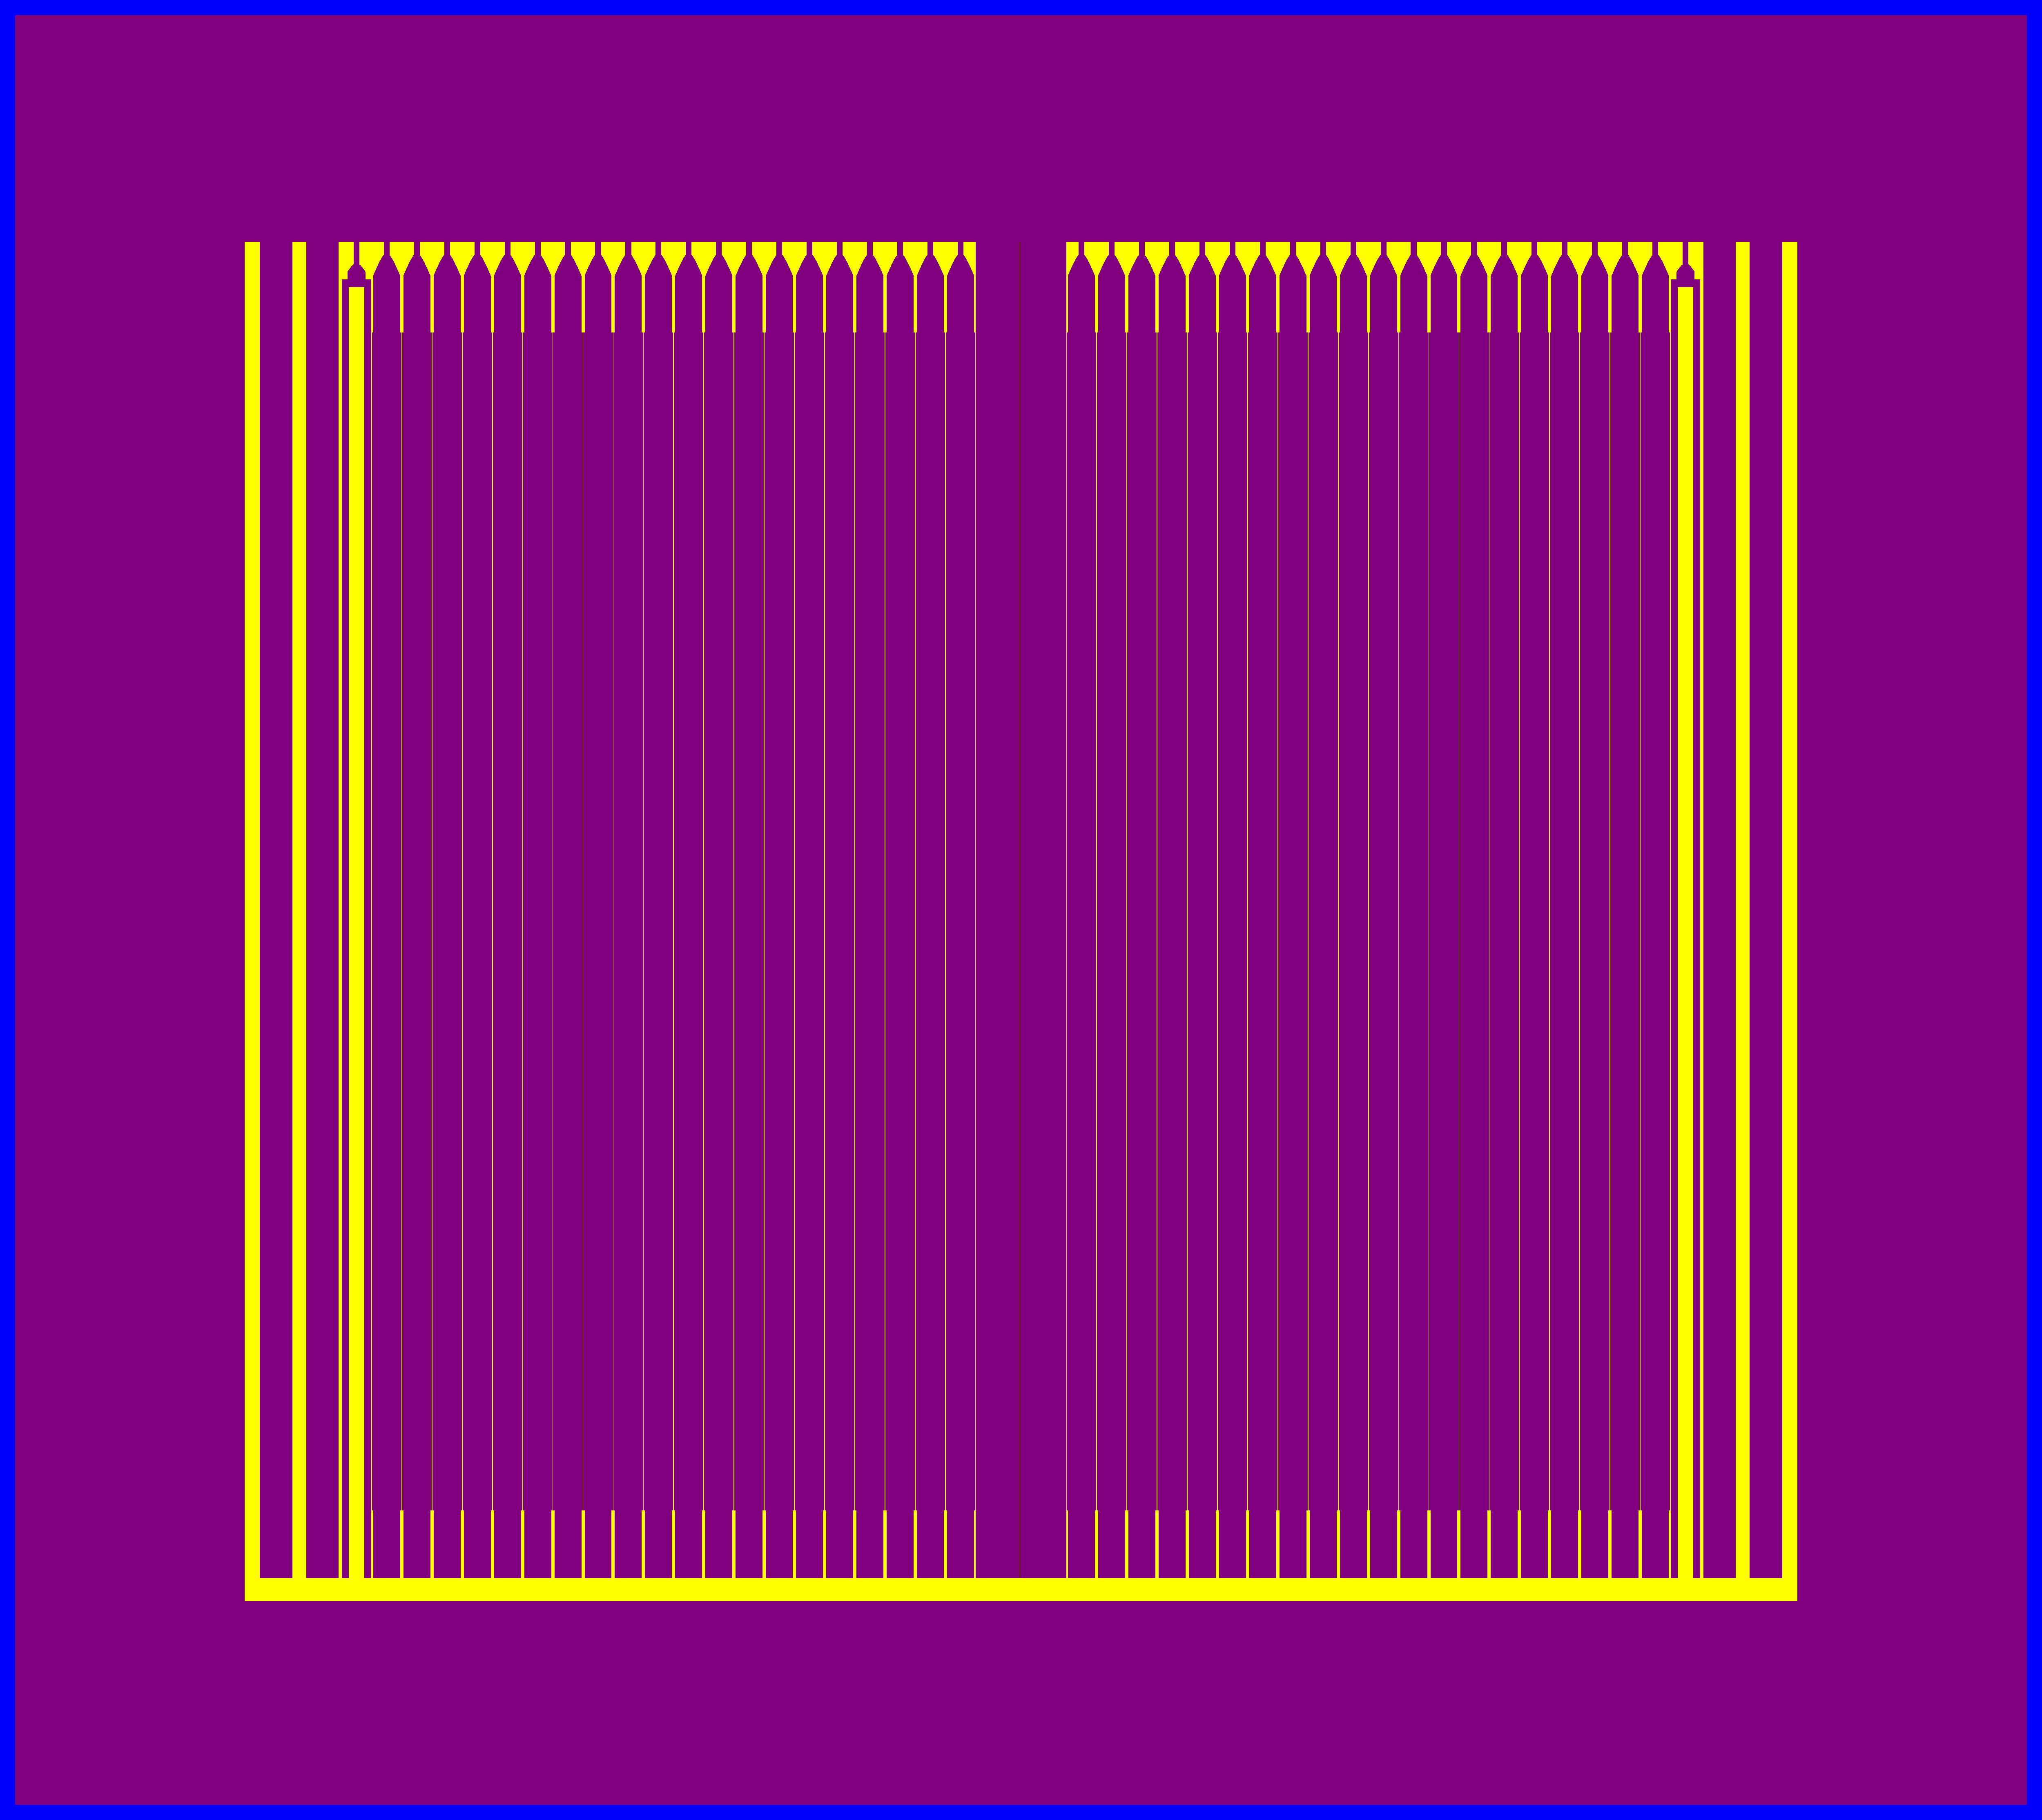
\includegraphics[width=0.5\linewidth]{figs/ch4/msbr_full_xz_openmc.png}
        \label{fig:msbr_model_xz}
    }
    \caption[Full core views of MSBR reference design and virtual model]{
        \subref{fig:msbr_ref_xy} Top down view of \Gls{msbr} reference design.
        \subref{fig:msbr_model_xy} Top down view of \Gls{msbr} CSG model.
        \subref{fig:msbr_ref_xz} Top down view of \Gls{msbr} reference design.
        \subref{fig:msbr_model_xz} Top down view of \Gls{msbr} CSG model.
    }
\end{figure}

As seen in figure \OpenMC and \SerpentTWO \Gls{msbr} models of reproduce these systems with
several approixmations. I will describe each reactor system, as well as any
relavant changes or approximations made in the model.

\subsection{Fuel salt}
\label{sub:msbr-fuel-salt}
The fuel salt used in the reactor core is
\ce{^{7}LiF}-\ce{Be}\ce{F_2}-\ce{Th}\ce{F_4}-\ce{U}\ce{F_4} at a concentration
of 71.7-17-12-0.3 mol-\%. The atom-\% for each nuclide is given in table\ldots 
\begin{table}[htpb] 
    \centering 
    \caption{Software tools that can model \Gls{msr} depletion with fuel reprocessing} 
    \label{tab:msbr_fuel_salt}
    \begin{tabulary}{\linewidth}{|C|C|C|C|} 
        \hline
        Nuclide & atom-\% & mass-\% \\
        \hline 
        \ce{Li} & 35.85 & \\
        \hline
        \ce{^{19}F} & 56\frac{107}{300} \approx 56.35 & \\
        \hline 
        \ce{^{9}Be} & 5\frac{1}{3} = 5.\overbar{3} & \\
        \hline 
        \ce{Th} & 2.4 & \\
        \hline
        \ce{U} & 0.06 & \\
        \hline
    \end{tabulary}
\end{table}

\subsection{Reactor core}
\label{sub:msbr-core}
The \Gls{msbr} core is split into three distinct different zones; zone I, zone
II, and the reflector zone.

\paragraph{Zone I} Zone I is the central-most region of the core, and is 13\%
fuel salt by volume. Zone I is divided into three subzones: zone I-A, zone I-B,
and the control rod zone. (more about these zones)

\paragraph{Zone II}


\paragraph{Reflectors}

\subsection{Vessel}
\label{sub:msbr-vessel}

\subsection{Reprocessing system}
\label{sub:msbr-reprocessing-system}

\section{OpenMC model}
\label{sec:openmc_model}

The \OpenMC \Gls{msbr} model reprocues the entire core region and the vessel
of the \Gls{msbr} with several approximations.

